\documentclass[11pt,a4paper]{article}
\usepackage{clrscode}
\usepackage[conEntregas]{tp2}
\usepackage[spanish]{babel} % para que comandos como \today den el resultado en castellano
\usepackage{a4wide} % márgenes un poco más anchos que lo usual
\usepackage[T1]{fontenc}
\usepackage{textcomp}
\usepackage{graphicx}
\usepackage{hyperref}
\usepackage{enumitem}
\newcommand{\subscript}[2]{$#1 _ #2$}
\usepackage[utf8]{inputenc} 
\usepackage{pdfpages}
\usepackage{amsmath}
\usepackage{vmargin}
\setpapersize{A4}


\begin{document}
\titulo{Trabajo Práctico 2}
\subtitulo{Modelando problemas problemas con grafos}

\fecha{\today}

\materia{Algoritmos y Estructura de Datos III}

\integrante{Buceta, Diego}{001/17}{diegobuceta35@gmail.com}
\integrante{Springhart, Gonzalo}{318/17}{glspringhart@gmail.com}
% Pongan cuantos integrantes quieran

\maketitle

\newpage
%\includepdf[pages={1,2}]{tp1.pdf}

\section{Introducción al problema}
\section{Justificación teórica}
\section{Algoritmos presentados}
\subsection{Kruskal}
\begin{codebox}
  \Procname{$\proc{KruskalSinPathComp}(ListaIncidencia: grafoCompleto, cantNodos: entero)$}
\li padre $\gets$ vector de enteros de tamaño de cantNodos y cargado con el valor de su posición en cada posición
\li AGM $\gets$ lista de incidencia vacia, de tamaño cantNodos-1
\li OrdenarPorPeso(grafoCompleto)
\li \For e:Arista $\in$ grafoCompleto 
\li \If $getPadre(indice(e.primerNodo), padre) $=$ getPadre(indice(e.segundoNodo),padre)$ \Then
\li agregar(e,agm)
\li \End
\li \End
\li Devolver AGM
\end{codebox}

\begin{codebox}
\Procname{$\proc{getPadre}(entero: indice, padre: vector de enteros)$}
\li \If $padre[indice] == indice$ \Then
\li Devolver indice
\li \Else
\li getPadre(indice(padre[indice]),padre)
\li \End
\end{codebox}


\begin{codebox}
\Procname{$\proc{getPadreConPathComp}(entero: indice, padre: vector de enteros, altura:vector de enteros, nivelesSubidos: entero$}
\li \If $padre[indice] == indice$ \Then
\li altura[indice] = nivelesSubidos
\li Devolver indice
\li \Else
\li padre[indice] = getPadreConPathComp(indice(padre[indice]),padre,altura,nivelesSubidos+1)
\li Devolver padre[indice]
\li \End
\end{codebox}


\begin{codebox}
\Procname{$\proc{unirPadres}(indiceNodo1: entero, indiceNodo2:entero, padre: vector de enteros)$}
\li padreNodo1 $\gets$ getPadre(indiceNodo1, padre)
\li padre[indiceNodo2]=padreNodo1
\end{codebox}

\begin{codebox}
\Procname{$\proc{unirPadresConPathComp}(indiceNodo1: entero, indiceNodo2:entero, padre: vector de enteros, altura:vector de enteros, nivelesSubidos: entero)$}
\li padreNodo1 $\gets$ getPadreConPathComp(indiceNodo1, padre,altura,0)
\li padreNodo2 $\gets$ getPadreConPathComp(indiceNodo2, padre,altura,0)
\li padreMenosAltura $\gets$ min(altura[padreNodo1],altura[padreNodo2])
\li padreMasAltura $\gets$ max(altura[padreNodo1],altura[padreNodo2])
\li padre[padreMenosAltura]=padreMasAltura
\end{codebox}


\begin{codebox}
\Procname{$\proc{armarGrafoCompleto}(nodos:vector de Nodos)$}
\li listaAristas $\gets$ inicializar lista de incidencia
\li matrizAristas $\gets$ inicializar matriz de adyacencia
\li \For $i \gets 0$ \To $tam(nodos)$
\li 	\For  $j \gets i+1$ \To $tam(nodos)$
			\li armar arista con datos de v[i] y v[j]
			\li agregar arista a listaAristas
		\End
	\End
\li armar matriz de adyacencia con la lista de incidencia
\li Devolver Matriz de adyacencia y Lista de incidencia
\end{codebox}

\begin{codebox}
\Procname{$\proc{retirarEjesInconsistentes}(listaAristas:lista incidencia, \sigma_{T}, profVecindario, f_{T}, forma, cantidadDeClusters, padre: vector de enteros )$}
\li \For $e:listaAristas$
\li calcular media y desviacion respecto del vecindario de profVecindario de profundidad de cada extremo de e. (usando una modificación de BFS)
\li si es inconsistente
\li sacar e de las listas
\li recorrer en la lista de ady todos los nodos alcanzables de uno de los extremos y modificar su representante en padre con cantidadDeClusters (usando una modificación de BFS)
\li aumentar en 1 el valor de cantidadDeClusters

\li \End
\end{codebox}

\subsection{Complejidad}

\subsubsection{Noción de eje inconsistente}
Para buscar ejes inconsistentes vamos a aprovechar las ventajas que nos brindan las implementaciones de listas de adyacencia y incidencia. \\
La idea es la siguiente: vamos a recorrer todas las aristas, sacándolas de la lista de incidencia y calcular con un método parecido a BFS los promedios de longitud de vecino, desviaciones, etc. Hay m aristas (que por estar trabajando con un AGM son $\approx$ n) y por cada una calcular esas cosas es O(m n+) $\approx$ O(n). En caso de ser considerado consistente vamos a recorrer, también con algo parecido a BFS, los nodos alcanzables desde uno de los extremos de la arista considerada inconsistente y le vamos a modificar su representante, con un vector de n posiciones donde en la posición i-ésima está el representante del nodo i-ésimo. Por temas de implementación, si la arista es inconsistente vamos a eliminarla de la siguiente forma: en la lista de incidencia modificamos su indice a -1, que es un valor que consideramos internamente como arista no disponible, y en la lista de adyacencia sí la eliminamos, accediendo en tiempo constante a la posicion del vector de ese nodo y con un iterador recorriendo sus nodos vecinos hasta encontrar el que corresponde con el otro extremo de la arista. Esto cuesta O(m) $\approx$ O(n), porque para cada nodo se recorre a lo sumo su grado y si se hace para todos los nodos será la suma de los grados de los nodos que es asintóticamente m, que por ser un árbol es O(n).\\
La complejidad total sería O($n^{2}$). Usar ambas listas nos permite tener los beneficios de recorer y 'deshabilitar' si es necesario las aristas en tiempo constante por la lista de incidencia y utilizar una modificación de BFS para poder calcular lo necesario y reasignar los representantes en caso de ser necesario de forma óptima por la lita de adyacencia.

\subsubsection{Procesamiento de puntos en el espacio}
Una vez leídos y almacenados en un vector todos los puntos del espacio ingresados, se procesarán uno a uno utilizando el siguiente procesamiento: por cada uno de ellos se recorrerán todos los que vengan después (en orden de ingreso). Esto nos asegura que cada nodo estará conectando con todos los demás (excepto él mismo) y así conseguiremos el grafo completo que tiene como nodos a los puntos ingresados. Esto lo conseguimos con complejidad O($n^{2}$). Construimos con esto la lista de incidencia y matriz y lista de adyacencia.\\
Para generar el AGM de kruskal, tenemos funciones que permiten facilitar el entendimiento del pseudocódigo correspondiente. Básicamente se procesa cada arista de la lista de incidencia del grafo completo, previamente ordenadas ( ordenada con el sort de C++ en O($\log{m}$ * m), donde m $\approx$ $n^2$), y se comprueba si la arista tomada actual (que es la de mínimo peso) genera un ciclo en las ya agregadas. Esto se hace mediante una implementación de funciones de UDS (Union Disjoint Set) que nos permite la manipulación de conjuntos de cosas disjuntas como las componentes conexas de un grafo. Una de estas funciones permite encontrar el representante de un punto/nodo (inicialmente cada nodo es su propio representante), lo que sería equivalente a preguntar a que componente conexa corresponde y en caso de ser de diferentes se agrega la arista, si no se sigue a la siguiente. Si la arista se elige se deben actualizar los representantes. Vamos a representar a los nodos en árboles y cada padre será el representante de un nodo, excepto la raíz que será su propio padre. Para mejorar la eficiencia, vamos a almacenar además del padre de cada nodo su altura. Imaginemos que cada representante sería la raíz de un árbol y al momento de buscar el representante de una de los hijos, 'subiríamos' hacia arriba preguntando por el padre de ese nodo, que en caso de no ser la raíz no será su propio representante y nos enviará hacia su padre. Este padre si no es la raíz, tampoco tendrá como representante a él mismo y nos enviará a su representante, así hasta llegar a la raíz. Durante toda esta búsqueda vamos a hacer dos cosas: se actualizará al nodo actual el representante y además se actualizará la altura del nodo que busquemos su representante, aumentando en 1 cada vez que subíamos un nivel en el árbol. Almacenar estas cosas nos sirve para: en primer lugar, la próxima vez que preguntemos por el representante de algún nodo de ese árbol no será necesario realizar otra vez todo ese recorrido (Path compression) porque estarán actualizados los representantes, y por otro lado al momento de unir las componentes conexas, tenemos podemos 'colgar' el árbol más chico del otro, realizando menos operaciones. Además la complejidad de buscar un representante será a lo sumo la altura del árbol (de a lo sumo n nodos) al que pertenece.\\
Así, al momento de unir las componentes conexas, simplemente actualizamos el representante del árbol más chico ( O(encontrar representante(nodo) $\approx$ O(altura árbol(nodo)) con el más grande. Entonces buscar un representante y unir componentes $\in$ O(log n).
\\Siguiendo con la explicación, el procesamiento de todas las aristas ( donde m = $\approx$ $n^{2}$)sería O($n^2$ * $\log$ n + $\log$ $n^{2}$ * $n^{2}$) $\approx$ O($\log$ $n^{2}$ * $n^{2}$) $\approx$ O($\log$ $n$ * $n^{2}$).
\section{Experimentación}
\subsection{Variaciones}
\begin{verse}
Tomaremos los casos de test brindados en http://cs.joensuu.fi/sipu/datasets/ y correremos nuestro algoritmo para poder obtener las clusterizaciones.\\
Los experimentos estarán centrados en analizar las diferentes tipos clusterizaciones que pueden realizarse variando las definiciones de eje inconsistente. Intentaremos analizar las configuraciones necesarias para que se pueda alcanzar una clusterización lo más cercana a la de la percepción humana y los resultados interesantes al que pueden llegarse. Para cada clusterización utilizaremos como solución previa los AGM obtenidos por los algoritmos de Kruskal, Kruskal con path compression y Prim, y a su vez indicaremos en cada caso las mediciones de tiempo correspondientes.  Para ello usaremos la porción de código utilizada en clase para medir tiempos con una cantidad de tres repeticiones de cada uno para una mejor precisión.\\

Dados los siguientes: $f_{T}$ multiplicador del promedio, $\sigma_{T}$ multiplicador de la desviación, y la profundidad del vecindario de los extremos del eje candidato, W(XY) el peso del eje candidato, y sea X e Y sus nodos extremos, definiremos un eje inconsistente:
\begin{itemize}
\item Forma 1: $\frac{W(XY)}{Promedio(Vecindario(X))}$ $>$ $f_{T}$ $  y $ $\frac{W(XY)}{Promedio(Vecindario(Y))}$ $>$ $f_{T}$, \\Es decir, la proporción entre el peso del eje candidato y el promedio de peso del vecindario de sus extremos es mayor al coeficiente dado.
\item Forma 2: $W(XY) >  Promedio(Vecindario(X)) + \sigma_{T}$ $ * $ $ desviacion(Vecindario(X)) $ $ y$ $W(XY) >  Promedio(Vecindario(Y)) + \sigma_{T}$ $ * $ $ desviacion(Vecindario(Y)) $, \\Es decir, que el peso del eje candidato supere al promedio del vecindario de sus extremos por al menos $\sigma_{T}$ unidades de la desviación del vecindario del extremo, y además se cumpla la forma 1.
\end{itemize}



Comencemos señalizando que la clusterización no es un problema matemáticamente definido y por ello podemos definirlo de forma tal que se obtenga diferentes resultados para mismas situaciones. 
La clusterización es la organización y detección de patrones en nuestros datos en grupos que tengan algún significado. Por lo general, a partir de un lote de datos, se busca caracterizarlos en base a la información que se pueda obtener de ellos y no por un patrón o clase de datos conocida dada. Es decir, no se separan los datos en función de su característica en propiedades o atributos previamente fijados, sino que se evalúa la correlación de cada uno de ellos entre todos los datos y en función de esto se agrupan. Estos analisis suelen dividirse como analisis supervisado y no supervisados (o clusteing), donde en los supervisados se cuenta inicialmente con las caracterizaciones que se esperan obtener y se analizan los datos para el reconocimiento de los patrones que permitan situarlo en el modelo correcto. Algunos ejemplos son redes neuronales, árboles de decisión, etc. Discutir el significado de correlación y significancia depende en gran medida de la naturaleza de los datos que se organicen. En nuestro caso, tenemos datos númericos correspondientes a puntos en el plano y en donde vamos a tomar como relación primaria entre ellos como su distancia euclídea. Experimentaremos con casos ya conocidos de clusterización y evualuaremos fuertemente la habilidad del modelo y sus parámetros para acercarse a los resultados de nuestra percepción, aunque siempre teniendo en mente la literatura del problema de clusterización y particularmente los analisis de los principios de agrupación propuestos por la filosofía de Gestalt previamente analizados.\\
Además, vamos a referirnos al método utilizado para la generación del AGM para referirnos a una determinada clusterización. Vamos a utilizar los datasets provistos por: \url{http://cs.joensuu.fi/sipu/datasets/}

\subsection{Experimentación}

\begin{verse}
Comenzaremos la parte de experimentación exponiendo algunos casos particulares de lo que se trata la clusterización.
\begin{center}
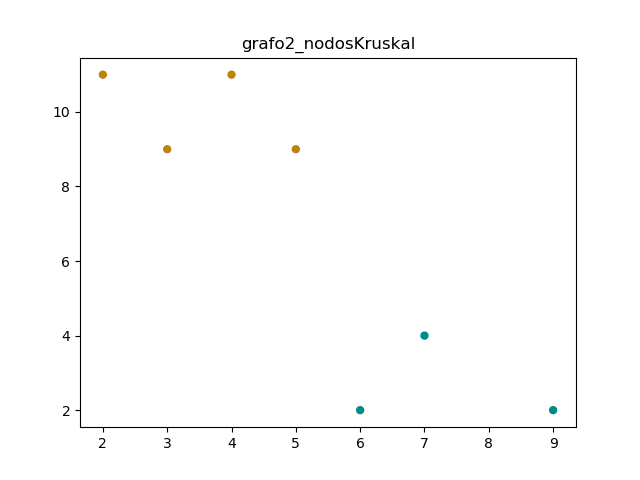
\includegraphics[scale=.8]{graficos/grafo2_nodosKruskal.png}
\end{center}
Intuitivamente los colores marcan ciertas diferencias entre los conjuntos de puntos. A simple vista los  naranja no parecen ser del mismo tipo que los azules, aunque habría que definir que significa eso técnicamente. En este caso estamos suponiendo que dos uniones de puntos que tengan distancia diferente son de diferente tipo. En este caso 'distancia diferente' significa una diferencia del doble de largo. Pero esta claro que en otro contexto dos cosas diferentes necesiten ser 'más' diferentes y la diferencia tenga que ser por ejemplo del triple y entonces acá no habría más que un grupo de puntos. Pero también podría ser lo contrario y considerar que dos puntos separados por una distancia muy chica ya son de diferente tipo y entonces podríamos conseguir que cada punto sea de un tipo diferente. A todo esto podemos involucrar las desviaciones que existen entre vecinos de puntos, porque podríamos querer ser un poco más restrictivos respecto de que separar, puede que en nuestro contexto nos importe cómo están distribuidos los vecinos de un punto más allá de las distancias que los separen. 
\begin{center}
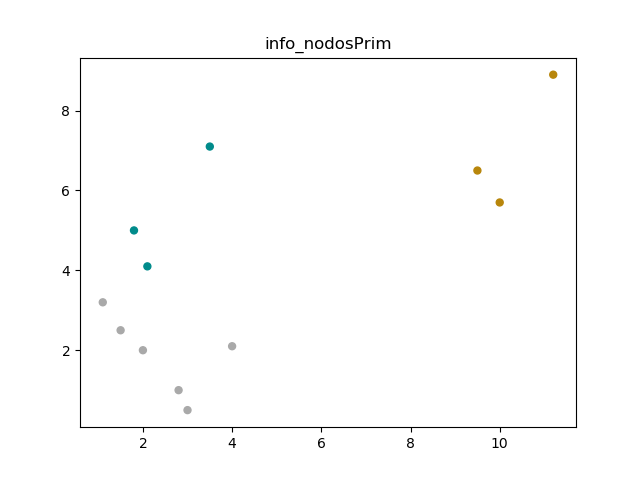
\includegraphics[scale=.8]{graficos/info_nodosPrim.png}
\end{center}
Por ejemplo en este caso, del lado izquierdo tenemos una serie de puntos que no parecen estar lo suficientemente alejados y sin embargo las desviaciones entre sus vecinos nos permiten ser más restrictivos con la medición.
\end{verse}

Con esta breve introducción, planteamos algunos interrogantes que pueden surgir y que sería interesante investigar en un análisis más profundo y completo de una mayor variedad de casos.

\subparagraph{Cómo conseguir clusters parecidos a nuestra percepción? Es siempre posible? Cómo varían los diferentes métodos de búsqueda de AGM para la clusterización? Como afectan a la clusterización la variación de los parámetros definidos para considerar un eje inconsistente?}


\subsection{Dataset: Aggregation}
\begin{center}
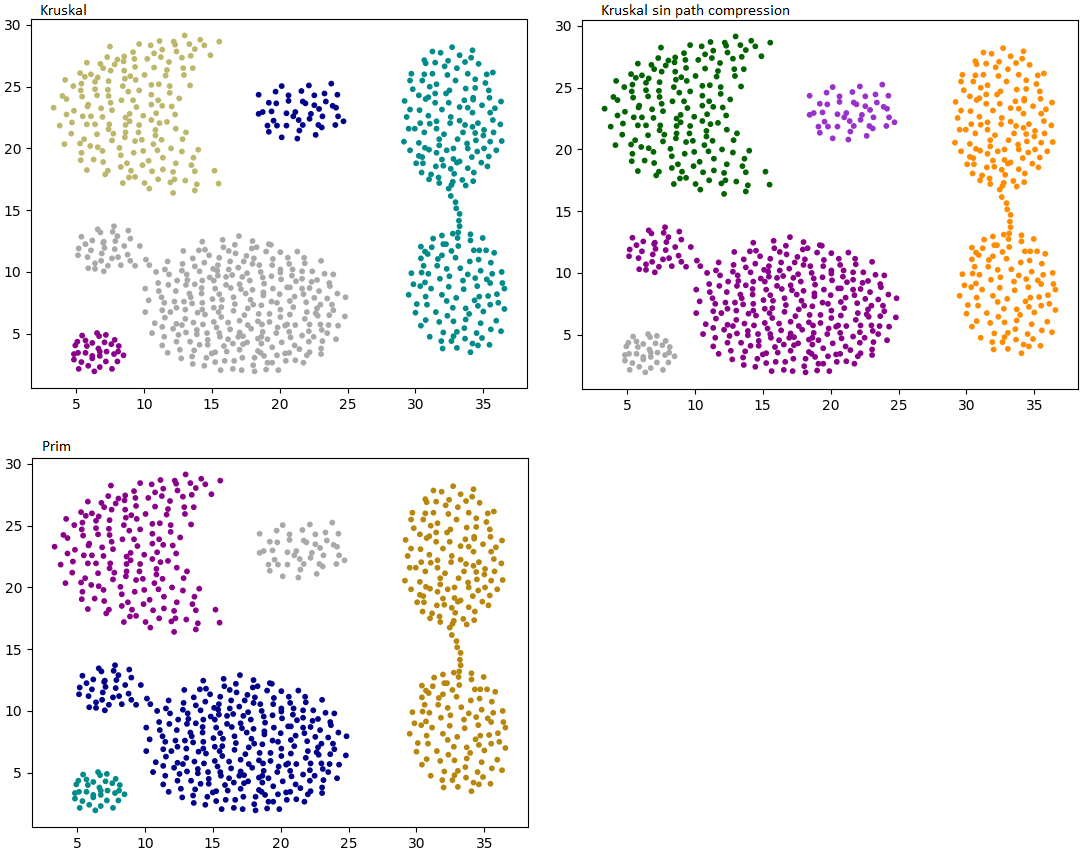
\includegraphics[scale=.5]{graficos/aggregation.png}
\end{center}

\subsubsection{Tiempos}
\begin{table}[ht]
\caption{Tiempos de ejecución en milisegundos} % title of Table
\centering % used for centering table
\begin{tabular}{c c c c} % centered columns (4 columns)
\hline\hline %inserts double horizontal lines
Cant.Puntos & Kruskal & Kruskal sin path comp & Prim \\ [0.5ex] % inserts table
%heading
\hline % inserts single horizontal line
788 & 254.66 & 386.66 & 151.66 \\ [1ex] % [1ex] adds vertical space
\hline %inserts single line
\end{tabular}
\label{table:nonlin} % is used to refer this table in the text
\end{table} 

Analizando el siguiente caso podemos ver que generando el AGM con cualquiera de los métodos elegidos obtenemos la misma clusterización. Elegimos como parámetros que un eje inconsistente debe superar en 2.5 al promedio de los vecinos de 2 pasos de sus extremos. La clasificación resulta en 5 clusters. Como primera observación, la percepción humana podría arrojar que el cluster de la esquina derecha en realidad podrían ser dos clusters diferentes, al igual que el cluster de la esquina izquierda. Si intentamos conseguir algo más cercano a esto, podemos intentar clasificar ahora también teniendo en cuenta la desviación. Como todos los puntos tienen una densidad de vecinos parecida, no tiene mucho sentido modificar la distancia del vecindario de los extremos (actualmente dos). Si reducimos el coeficiente del promedio de 2.5 hasta 1.4 y el coeficiente de la desviación lo fijamos en 2, d = 2. Después de varios intentemos, encontramos que en ese punto obtenemos lo siguiente:


\begin{center}
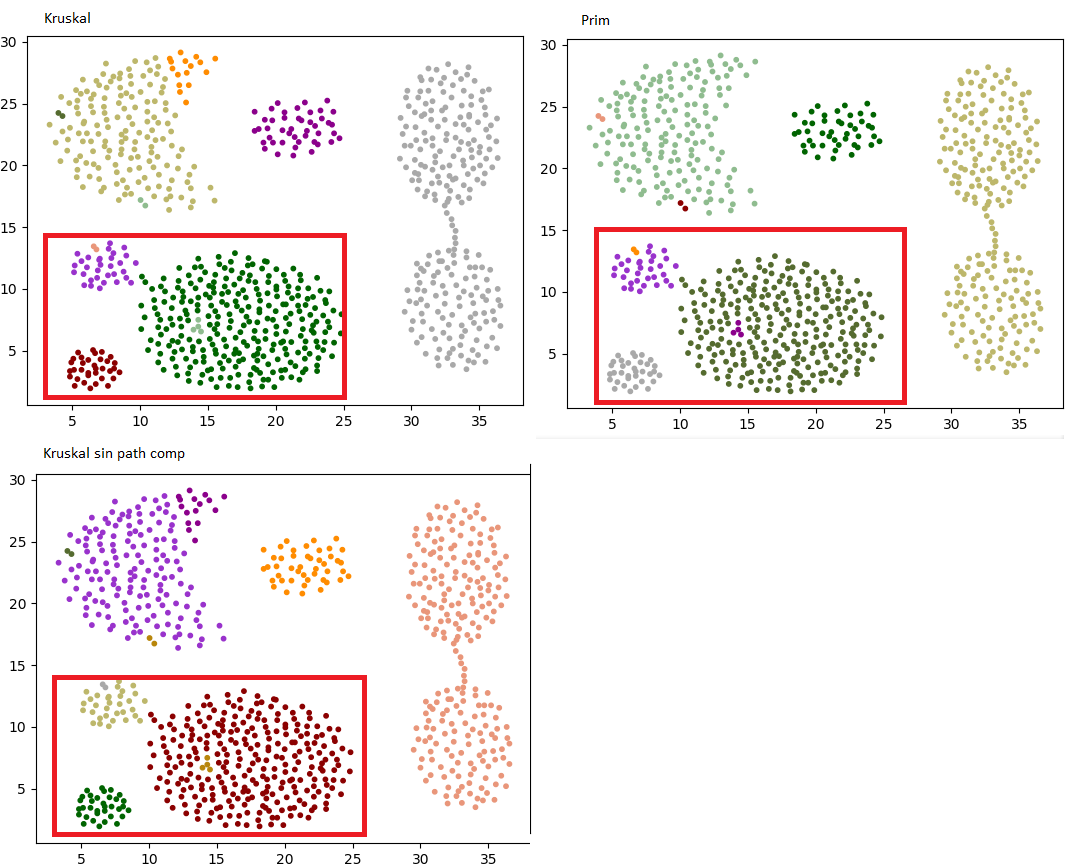
\includegraphics[scale=.5]{graficos/aggregation2.png}
\end{center}
\end{verse}

Por un lado, conseguimos auentar los clusters pero las modificaciones generan ciertas inconsistencias en zonas de puntos donde la clusterización estaba bastante cercana a nuestra percepción. Todo esto se da en un contexto en donde buscamos ejes inconsistente que cumplan con los requisitos anteriormente mencionados y el problema es que como se ha visto anteriormente, nuestra percepción suele utilizar en una serie de factores que no necesariamente se corresponden con un método de clusterización en cuestión. Por ello es posible y buscaremos en esta experimentación convencernos lo más posible que la clusterización puede variar lo suficiente con determinados cambios en los requisitos tomados para evaluar y su correspondencia con nuestra percepción puede estar notablemente alejada.
\\ En nuestro gráfico esto genera que nosotros veamos tres clusters bien definidos en la esquina inferior izquierda y nuestro método sólo detecta correctamente dos. En este caso la razón es muy simple, la unión de los conjuntos de puntos marcados en rojo esta formada por un 'cuello' que nuestra percepción ignora y por eso separamos los conjuntos en dos clusters diferentes. Mientras que computacionalmente, ese cuello no cumple nuestra noción de eje inconsistente y en caso de que tratemos de forzarlo comenzamos a tener estas inconsistencias, porque nada impide que otros dos puntos con características similares a este cuello se encuentren dentro de uno de los clusters y en ese caso, por la propia consistencia de nuestro método, también sería considerado inconsistente.\\
Otro punto interesante a considerar, es que para estos nuevos parámetros conseguimos diferentes clusterizaciones. Particularmente encontramos un mini-cluster en el cluster turquesa de Kruskal sin path compression y en Prim, y ausente en Kruskal. Esto proviene por como buscamos ejes inconsistentes -recorriendo las aristas del AGM- y cómo se construyeron los AGM. En la sección de algoritmos se explica el funcionamiento y sólo vamos a resaltar que entre Kruskal y Prim la generación es diferente, y mientras en Prim estamos construyendo todo el tiempo sobre el árbol actual, en Kruskal nos limitamos a guardar las aristas de menos peso que no generen circuito con las actuales y esto en algún paso k-ésimo no necesariamente es un árbol, excepto que k sea el último. Por otro lado, Kruskal sin path compression al agregar una nueva arista y unir las componentes conexas lo hace sin intentar optimizar esa acción, y esto puede generar que los referentes de una componente conexa de Kruskal sean diferentes a los de la misma componente conexa en Kruskal sin path compression.
Entonces una de las cosas que vamos a ver es si esto es realmente factible y entonces podemos utilizar esta técnica para poder ver a grandes rasgos los clusters y en función de nuestro interes enfocarnos en una zona en particular. Esto nos facilita porque al momento de volver a clasificar esa zona, lo haríamos restringiendo nuestro domino de patrones (anteriormente de todo el conjunto de puntos) hacia uno más pequeño.\\ 
Como primeras conclusiones podemos decir que en contextos en donde hay conjuntos de puntos con densidades similares y que existen ciertas uniones con desviaciones y promedios similares (recordemos que la desviación la calculamos entre los vecinos y por más que en ese cuello hay menos vecinos en comparación con algún punto en medio de un cluster en particular, como las distancias entre nodos son similares en ambos casos, la desviación y largo promedio en ejes también lo son)  esto hace que no se 'encuentren' ejes inconsistentes. 
\\

\subsection{Grafo r15}
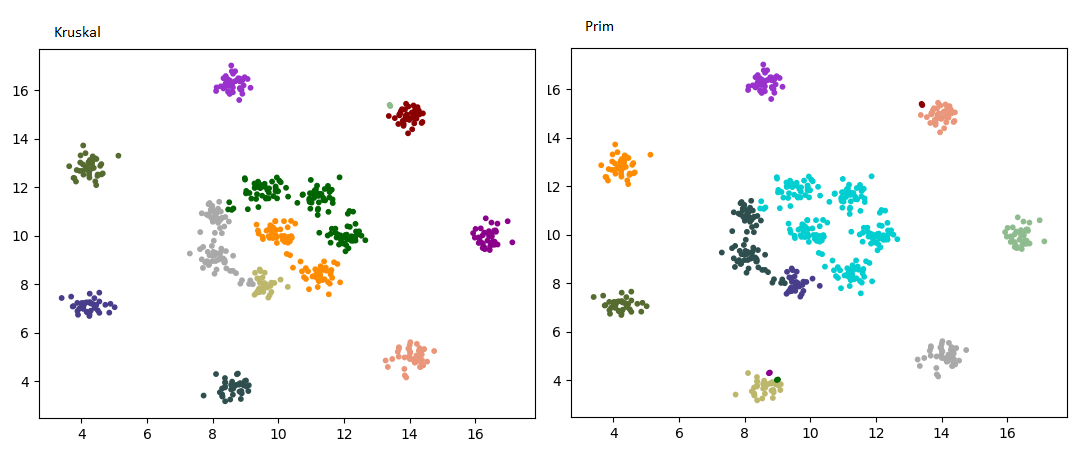
\includegraphics[scale=.5]{graficos/r15.png}
 Fijamos $\sigma_{T}$ $=$ 3.3 y $f_{T}$ $=$ 2.4, d = 2. Por razones de espacio evitamos poner a Kruskal sin path compression porque dan exactamente lo mismo.
 Los valores de los parametros fueron: factor de proporción en 1.8 y la desviación en 3.8. En este caso, pequeñas modificacione en el factor de proporción o desviación no generaban clusters diferentes. Sin embargo se puede apreciar cómo los clusters exteriores están definidos muy parecida a cómo sería esperable mientras que en el centro empiezan a juntarse puntos de -a nuestra percepción- diferente cluster. El problema es que al mirar con atención los posibles ejes que unen en el AGM los nodos que serían de diferente cluster cumplen ciertas cosas:
\begin{center}
 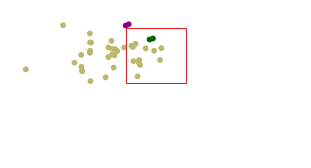
\includegraphics[scale=.7]{graficos/r15_zoom.png} 
 
\end{center}
Si hacemos un zoom a la zona del cluster marrón claro de Prim que tiene como dos clusters adicionales y no intuitivo para nuestra percepción, demarcamos la zona marcada con rojo y obsvervamos el caso del cluster verde es bastante visible que cualquier de los posibles ejes que los une (a los nodos) en el AGM va a cumplir tener mayor factor de proporción de promedio con respecto a los vecinos. Respecto de la desviación podría justificarse de un modo similar. Entonces podemos justificar de forma mas o menos razonable por qué se consideran - y bien- inconsistentes para nuestro modelo.
\\
Modifiquemos ahora un poco la forma de clusterizar. Fijemos d = 3, porque en este caso tiene sentido pensar que nos va a dar un poco de mayor consistencia en las mediciones, y utilicemos sólo la proporción entre ejes con $f_{T}$ $=$ 2.6.
\begin{center}
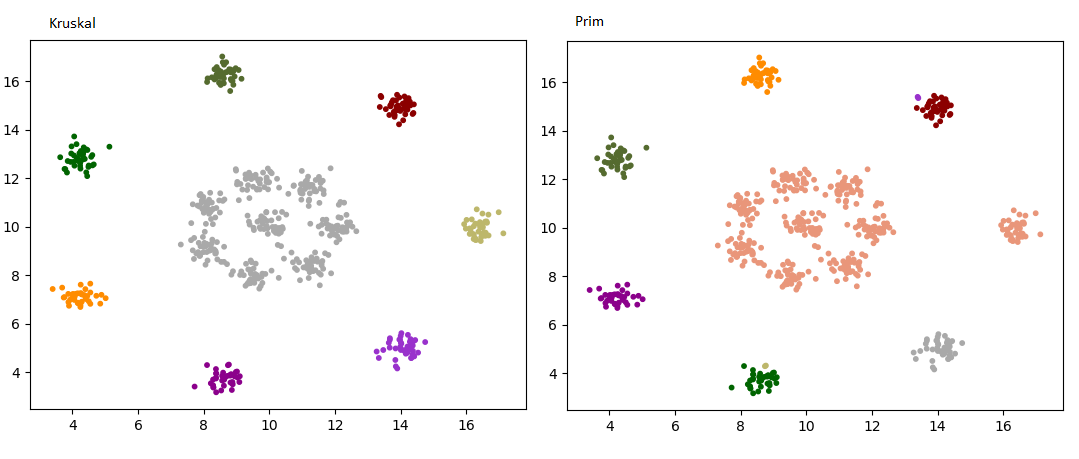
\includegraphics[scale=.5]{graficos/r15_2.png}
\end{center}
Como era esperado, el centro ahora se convierte en todo un gran cluster. Era algo esperado al agrandar los vecindarios, porque de esa manera por la densidad y distribución de los puntos de centro tiene sentido pensar que al tener en cuenta más vecinos será más complicado superar los 2.6 de proporción de eje. Si llegaramos a reducir el valor, es posible que obtengamos clusters no tan representantivos porque al sacar la desviación de consideración estamos sacando información útil para decidir si separar dos conjuntos de puntos más alla si existe algún eje lo 'suficientemente' largo.
\begin{center}
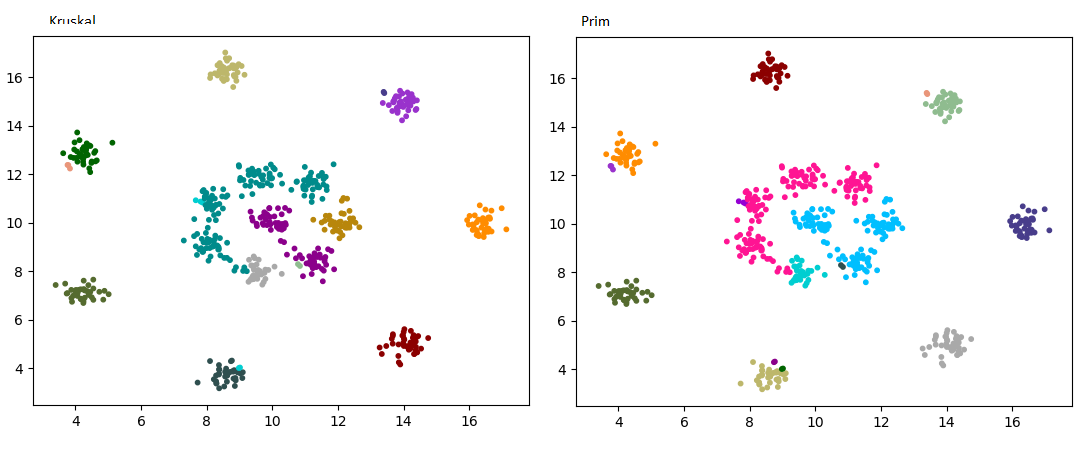
\includegraphics[scale=.5]{graficos/r15_3.png}
\end{center}
Efectivamente podemos ver que se encuentran más clusters debido a que como dijimos hay menos información con la cuál decidir, es decir, quizá dos nodos están suficientemente alejados pero por la dispersión de vecinos que tienen a nuestros ojos forman parte de lo mismo.\\
Para cerrar este tipo de contextos, encontramos que al igual que antes, Prim suele tender a generar clusters 'aislados' que intentaremos dar explicar viendo más casos y recopilando más información.
\\



\subsection{Dataset: Spiral}
\subsubsection{Tiempos}
\begin{table}[ht]
\caption{Tiempos de ejecución en milisegundos} % title of Table
\centering % used for centering table
\begin{tabular}{c c c c} % centered columns (4 columns)
\hline\hline %inserts double horizontal lines
Cant.Puntos & Kruskal & Kruskal sin path comp & Prim \\ [0.5ex] % inserts table
%heading
\hline % inserts single horizontal line
312 & 33 & 32 & 32.66 \\ [1ex] % [1ex] adds vertical space
\hline %inserts single line
\end{tabular}
\label{table:nonlin} % is used to refer this table in the text
\end{table} 


\begin{figure}[!htb]
   \begin{minipage}{0.45\textwidth}
     \centering
     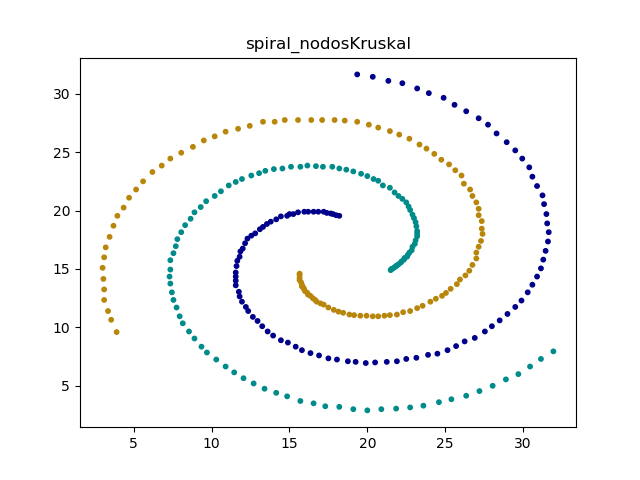
\includegraphics[scale=.5]{graficos/spiral_nodosKruskal.png}
   \end{minipage}\hfill
   \begin{minipage}{0.45\textwidth}
     \centering
     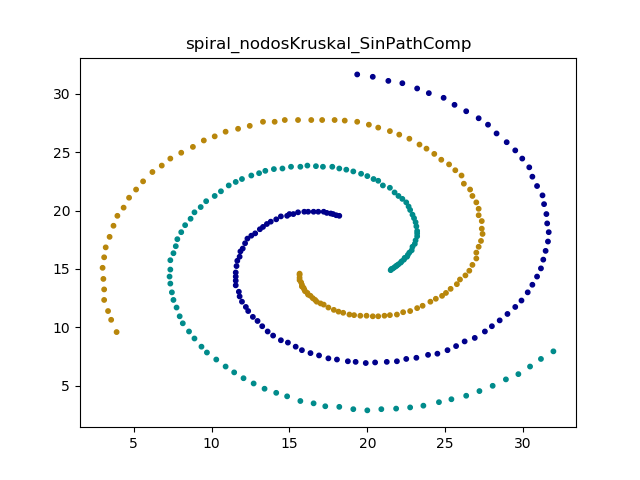
\includegraphics[scale=.5]{graficos/spiral_nodosKruskal_SinPathComp.png}
   \end{minipage}\hfill
   
\end{figure}

\subsubsection{Gráficos}
En este caso fijamos $f_{T}$ $=$ 3.3 y la profundidad del vecindario la fijamos en 2 y 3. Es razonable pensar que ambos AGM serán similares porque no hay demasiadas opciones de ejes para los nodos, porque cada una de las líneas de puntos tiene pocos vecinos cercanos (si pensamos en el grafo completo) con los cuales tiene sentido que se una formando una distancia mínima. Imaginemos el grafo completo y su conversión a AGM y pensemos que entre cada una de las líneas de puntos que vemos como clusters diferente existe una arista que las une (por ser un árbol) y si habría más de una seguro se podría encontrar un árbol generador con menor peso y esto sería absurdo porque Kruskal y Prim nos garantizan que lo consiguen, de modo que tiene sentido pensar que entre cada una de esas líneas existe sólo una arista que las une y que su peso es mucho mayor al de cualquiera de los demás ejes. Entonces al momento de experimentar, pensar en la profundidad de vecinos o proporción de eje inconsistente desde el detalle no tiene gran sentido, dado este caso donde las líneas están bien separadas no hay problemas para conseguir una separación de nodos intuitiva. \\


\subsection{Dataset: Pathbased}

\subsubsection{Tiempos}
\begin{table}[ht]
\caption{Tiempos de ejecución en milisegundos} % title of Table
\centering % used for centering table
\begin{tabular}{c c c c} % centered columns (4 columns)
\hline\hline %inserts double horizontal lines
Cant.Puntos & Kruskal & Kruskal sin path comp & Prim \\ [0.5ex] % inserts table
%heading
\hline % inserts single horizontal line
300 & 32 & 46 & 27 \\ [1ex] % [1ex] adds vertical space
\hline %inserts single line
\end{tabular}
\label{table:nonlin} % is used to refer this table in the text
\end{table} 

\subsubsection{Gráficos}
En este caso, tenemos algo similar al anterior pero tenemos una distribución de puntos que nos hace pensar que probablemente sea más dificil de encontrar una clusterización clara y tengamos que ajustar las desviaciones, el vecindario, y las proporciones de peso entre ejes. clusterización clara. 
\begin{center}
     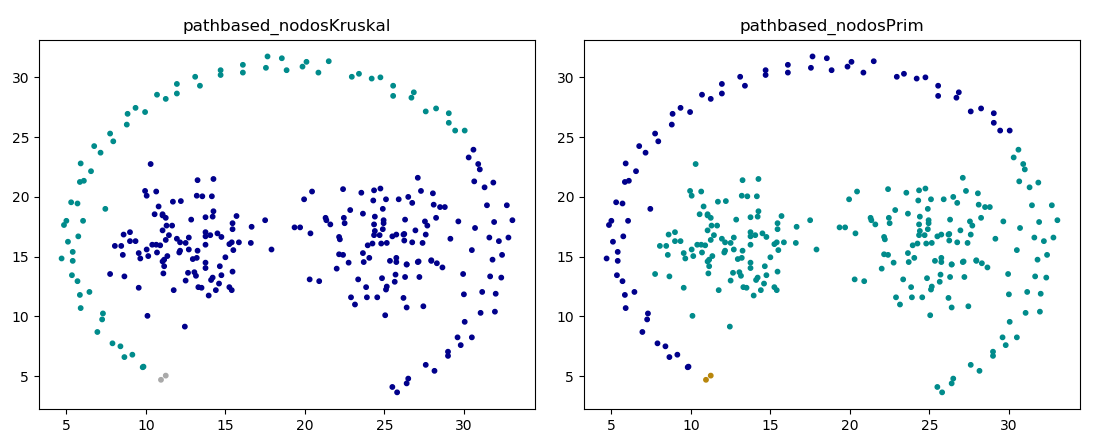
\includegraphics[scale=.5]{graficos/pathbased_nodosKruskal_nodosPrim.png}
\end{center}

Como vemos, fijando $f_{T} = 2.35$, d $=$ 3, lo que conseguimos no es lo que esperaríamos ver clusterizado. Es otro caso en donde la distribución de los puntos, la cercanía entre los clusters esperables, la relación con los pesos de los ejes del grafo, entre otras cosas, hacen que sea necesario trabajar un poco más para poder conseguir algo mejor.

\begin{center}
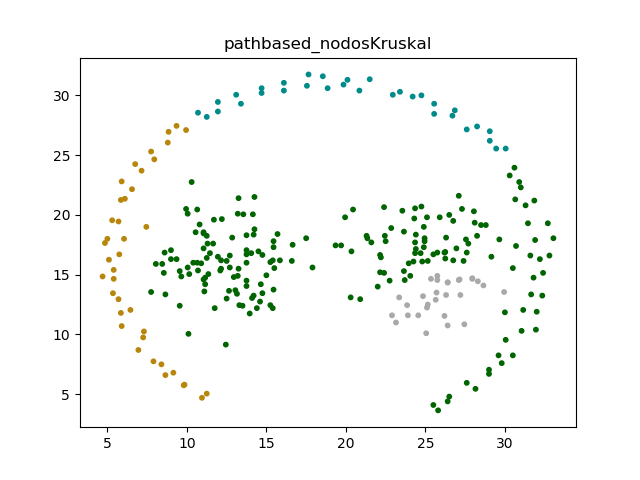
\includegraphics[scale=.5]{graficos/pathbased_nodosKruskal3.png}
\end{center}
Incluyendo ahora la desviación y ajustando un poco más los parámetros con $f_{T} = 1.9$, $\sigma_{T} = 2.5$ y d $=$ 2 tenemos algo que nos da más información para analizar.
Para que sea más fácil de ver lo señalamos en rojo y con un zoom a la imagen. Siempre es importante tener en la cabeza el posible AGM y a partir de ello analizar las razones por las que hay separaciones inesperadas de cluster.

\begin{center}
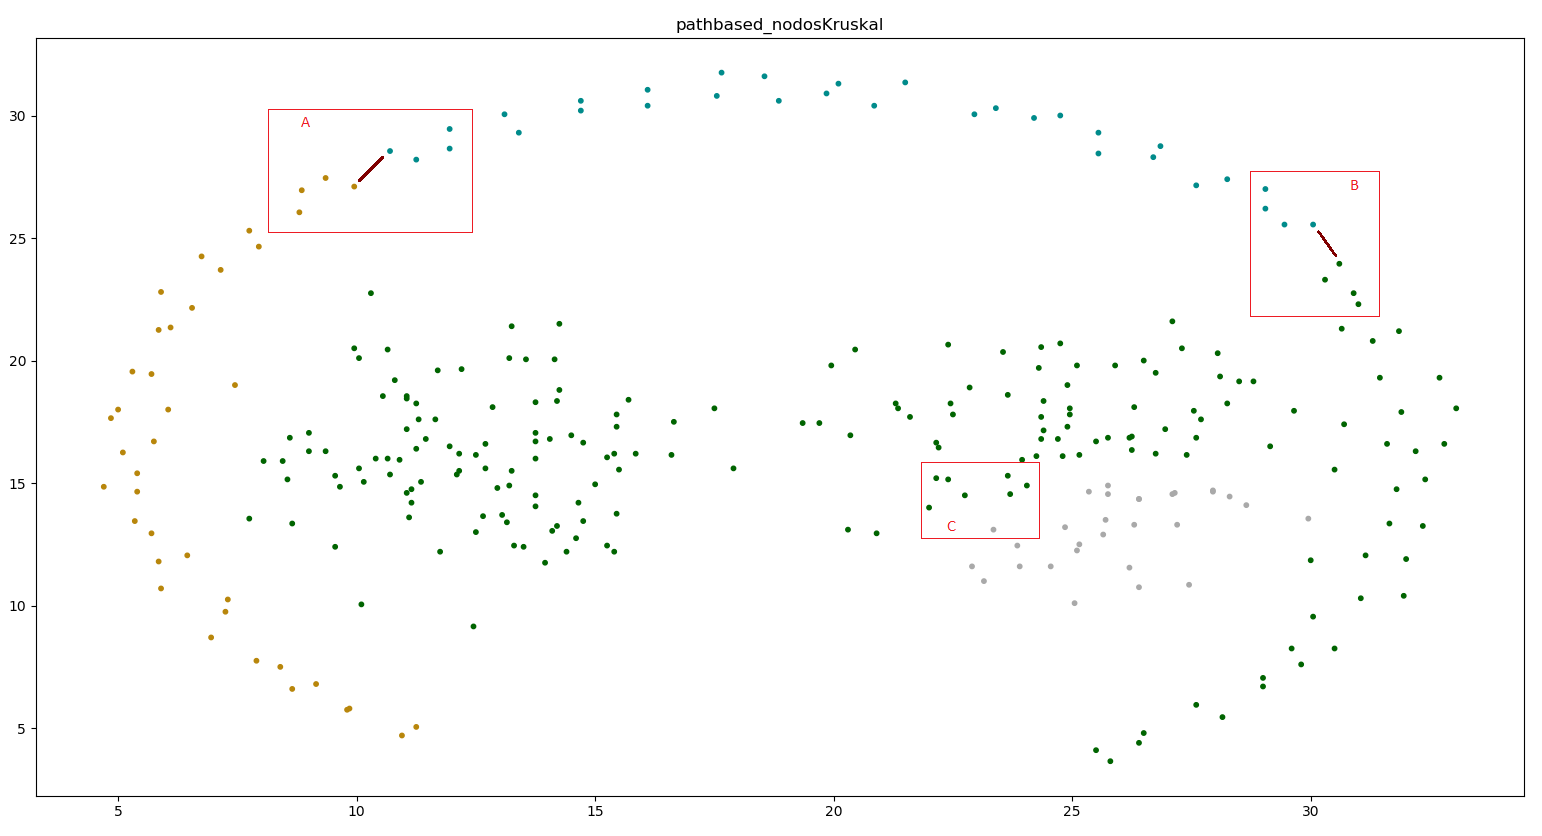
\includegraphics[scale=.41]{graficos/pathbased_nodosKruskal2.png}
\end{center}
El tema es claro: reducir el coeficiente de proporción de pesos nos genera clusters no esperados pero que si los analizamos en particular son correctos según nuestra medición. En las zonas señalizadas pusimos un eje bordo que simboliza la posible unión de los nodos en el AGM. Es claro que ese eje en proporción a los vecinos es superior y que para poder 'estabilizarlo' (en términos de evaluarlo y clusterizarlo como nosotros lo vemos) habría que tomar un vecindario más grande, posiblemente con d igual a 4 ó 5. En la zona C pasa algo similar y se le agrega algo: la distribución de puntos es diferente, lo cual genera que este tipo de situaciones sean difíciles de separar.


\subsection{Dataset: A1}
\subsubsection{Tiempos}
\begin{table}[ht]
\caption{Tiempos de ejecución en milisegundos} % title of Table
\centering % used for centering table
\begin{tabular}{c c c c} % centered columns (4 columns)
\hline\hline %inserts double horizontal lines
Cant.Puntos & Kruskal & Kruskal sin path comp & Prim \\ [0.5ex] % inserts table
%heading
\hline % inserts single horizontal line
3000 & 3839.66 & 5934.33 & 1939.33 \\ [1ex] % [1ex] adds vertical space
\hline %inserts single line
\end{tabular}
\label{table:nonlin} % is used to refer this table in the text
\end{table} 

\subsubsection{Gráficos}
En este caso tenemos una clusterización bastante evidente a simple vista sin embargo después de variar los parámetros lo más parecido que podemos conseguir es lo siguiente:
\begin{center}
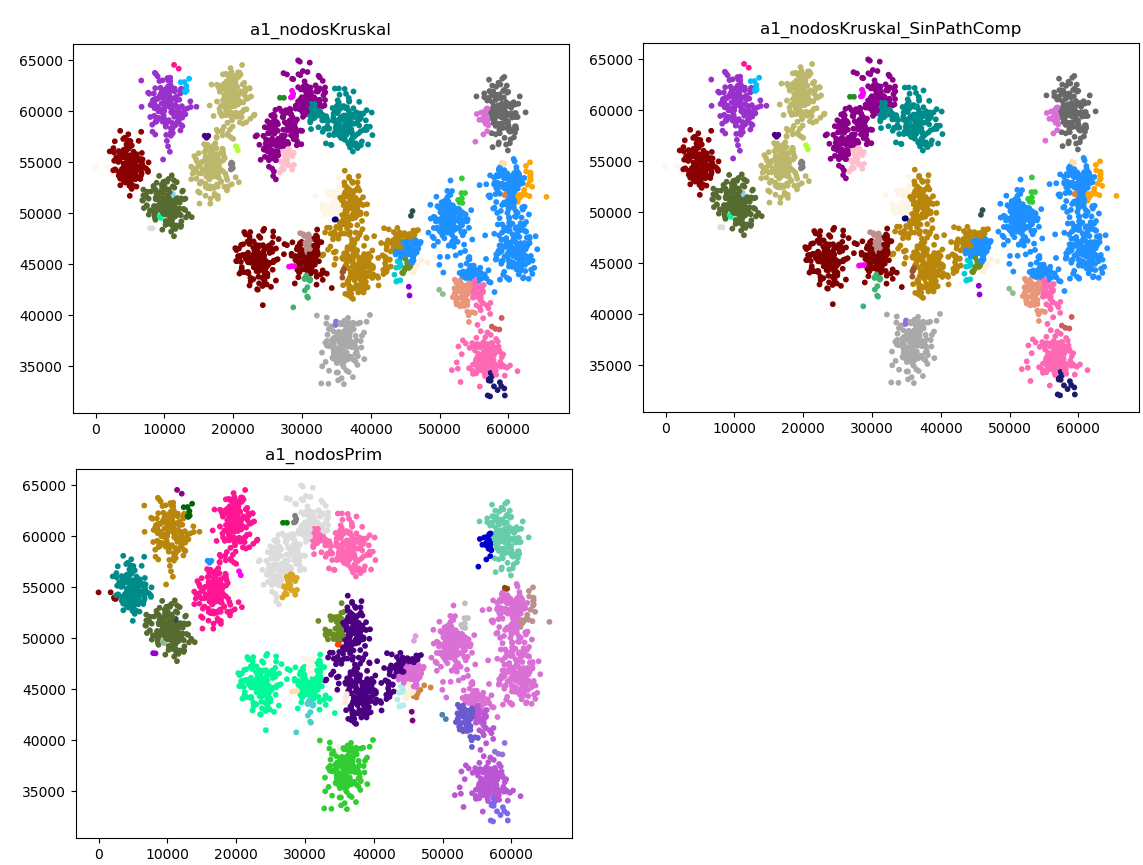
\includegraphics[scale=.41]{graficos/a1_nodosKruskal_Prim.png}
\end{center}
Volvemos a encontrar un factor que se viene repitiendo en los distintos datasets: la transición entre lo que a simple vista son diferentes clusters algorítimicamente no suele ser fácil de detectar. Modificando los parámetros podemos llegar a solucionar el problema en alguna zona en particular y al mismo romper lo anteriormente bien -a nuestra percepción- clusterizado. Un posible camino sería subdividir las áreas de puntos que queremos clusterizar y separarlas en función de patrones similares que permitan fijar los parámetros sin romper otras zonas ysa clusterizadas. Sin embargo en este caso en particular no es muy claro qué áreas subidividir.\\
Veamos otro caso en donde sería un poco más claro cómo dividir en caso de que pase esto.

\subsection{Dataset: Compound de Zahn}
\subsubsection{Tiempos}
\begin{table}[ht]
\caption{Tiempos de ejecución en milisegundos} % title of Table
\centering % used for centering table
\begin{tabular}{c c c c} % centered columns (4 columns)
\hline\hline %inserts double horizontal lines
Cant.Puntos & Kruskal & Kruskal sin path comp & Prim \\ [0.5ex] % inserts table
%heading
\hline % inserts single horizontal line
399 & 61 & 90.33 & 46 \\ [1ex] % [1ex] adds vertical space
\hline %inserts single line
\end{tabular}
\label{table:nonlin} % is used to refer this table in the text
\end{table} 
\subsubsection{Gráficos}
Fijando $f_{T} = 1.19$, d $=$ 2, $\sigma$ $=$ 4.3 encontramos lo siguiente: (por motivos de espacio y que los 3 AGM dan igual sólo ponemos 1)
\begin{center}
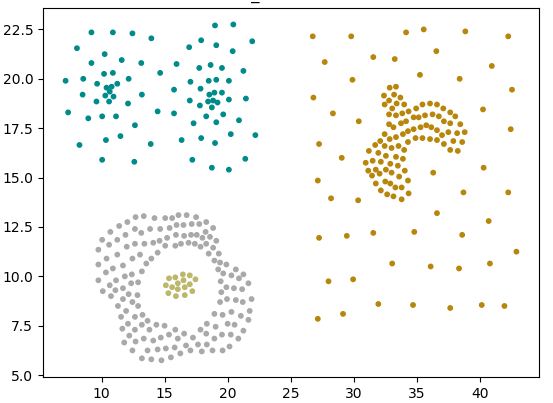
\includegraphics[scale=.6]{graficos/zahn.png}
\end{center}
Es claro que la clusterización obtenida está cerca de la esperada, aunque también sería esperable que los de la esquina superior izquierda sean dos diferentes y que el de la derecha también lo sea. Primero vamos a tratar de modificar los parámetros para obtenerlo y si no podemos vamos a intentar aplicar clusterizar por partes, porque acá sí es más claro que tenemos tres zonas que podemos tratar por separado.
\begin{center}
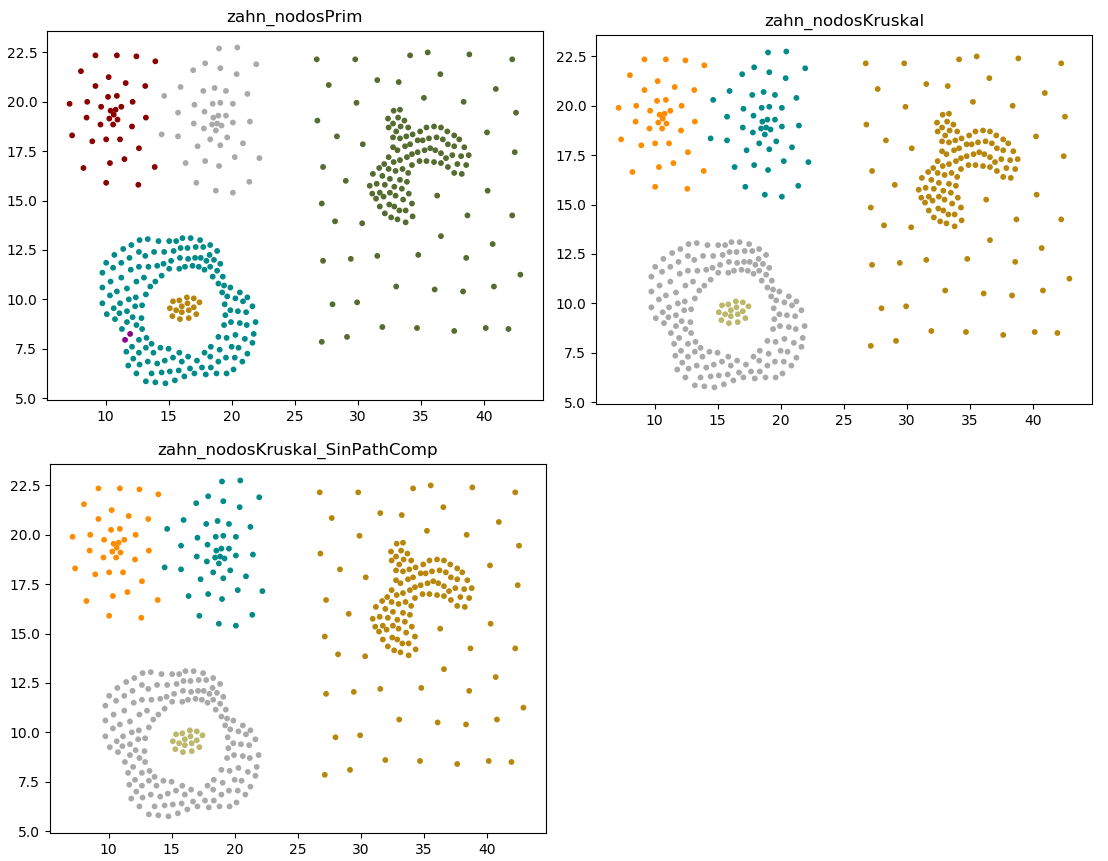
\includegraphics[scale=.55]{graficos/zahn_nodosPrim_Kruskal.png}
\end{center}
Si  miramos con atención, la solución que utiliza Prim generó un cluster adicional, mientras que Kruskal no, aunque ninguno pudo clasificar en dos la parte derecha de la imagen.\\
Intentemos probar ahora clusterizar esa parte sola, tomando a partir de x $>=$ 25 y ver si podemos clusterizarla y en cierto modo terminar clusterizar 'bien' todo el gráfico.
\begin{center}
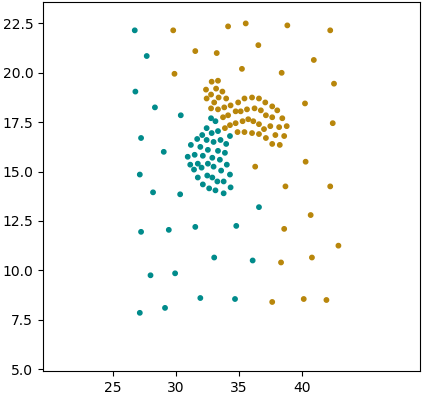
\includegraphics[scale=.6]{graficos/zahn_nodos2.png}
\end{center}
Obtuvimos está nueva clusterización fijando d $=$1, $\sigma$ $=$ 1.2, $f_{T}$ $=$ 1.2, y nuevamente nos encontramos con dificultades para poder separar grupos de puntos que sacándolos del contexto anterior parecía bastante sencillo de separar, los Gestalts principles se hacen presentes en casi todos los experimentos.\\

Retomando el gráfico anterior donde Prim generaba un cluster adicional a Kruskal, lo que hicimos fue hacer un zoom en esa región y análisis en detalle, marcando en rojo cuáles son las aristas que unen esos nodos en particular. Obtuvimos lo siguiente:
\begin{center}
\includegraphics[scale=.6]{graficos/zahn_conex_Prim.png}
\includegraphics[scale=.6]{graficos/zahn_conex_Kruskal.png}
\end{center}

Ambos métodos tienen diferentes técnicas para generar un AGM, esto es algo que no podemos controlar en profundidad en todos los datasets pero que en este en particular notamos, aunque es posible que en otros también ocurriese y no se notara porque no afectaba a la clasificación de los nodos. En este caso sí y se nota claramente en la imagen. Internamente, la arista en cuestión es la número 280 en Kruskal mientras que Prim la consiguió como arista 115. En Prim imaginamos que esta parte es la especie de 'hojas' del árbol y que la raíz está hacia la derecha. Marcamos con azul la arista que se considera inconsistente. En Kruskal aparentemente sería una situación inversa, estamos donde sería algo similar a la raíz y hacia el otro lado estaría esta situación. En la imagen es apreciable que al cambiar esas relaciones el vecindario también es diferente y en la zona que une Kruskal aumentan levemente los promedios de pesos de ejes y esto impide que sea considerado inconsistente.


\subsection{Conclusiones}
Durante la experimentación con diferentes tipos de conjuntos pudimos comprobar en persona las discusiones que tuvieron lugar en secciones previas de la introducción teórica. Vimos cómo son afectados los análisis en función de pequeños movimientos de los parámetros y la dificultad para encontrar una configuración que permita una clasificación cercana a nuestra percepción en todo su conjunto. En caso de tener que clusterizar diferentes gráficos se deberá necesariamente contar con el tiempo para una experimentación exhaustiva que permita realizarlo y en muchos casos la subdivisión de los gráficos para el tratado de zonas que presenten patrones de caracterización diferentes y estar preparados para no conseguir los clusters idénticos a lo esperado. 
\\ También cabe mencionar las diferentes técnicas de generación de AGM, donde por lo menos a nivel clusterización no hubo una diferencia considerable para alguno en la clusterización de algún conjunto en particular. Sí hay que mencionar las diferencias de performance evaluadas: es claro que más alla de la complejidad teórica Kruskal con path compression en la práctica es mucho mejor y en algunas situaciones es más notable que en otras. Además, en este trabajo en particular se construyó el AGM partiendo del grafo completo, lo que quiere que decir que una técnica como Kruskal en la que es necesario ordenar las aristas se ve altamente perjudicada. Otras forma consisten en calcular un grafo con los k-vecinos más  cercanos para cada nodo y de esta forma evitar partir de un grafo completo en donde m $\approx$ $n^{2}$.\\ En general, clusterizar en determinados casos requerirá aceptar cierto grado de error, debido a la falta de comprobación exacta de los resultados, y el contexto determinará cuán exacto y exhaustivo, respecto de una percepción esperada, deberán ser los métodos considerados para la clusterización.
\end{document}



